\section{Differential Calculus}

\begin{Theorem}{
    Fundamental Lemma\footnote{\href{https://trello.com/c/byu9Pyy8}{Calculus with Analytic Geometry by George F. Simmons}, p. 680}
    \phantomsection\hypertarget{fundamental-lemma}
}{fundamental-lemma}
    Suppose that a function $z = f(x, y)$ and its partial derivatives $f_x$ and $f_y$ are defined at a point
    $(x_0, y_0)$, and also through some neighborhood of this point. Suppose further that $f_x$ and $f_y$ are continuous
    at $(x_0, y_0)$. Then the increment $\Delta z$ can be expressed in the form of

    \begin{equation}
        \Delta z = f_x(x_0, y_0)\Delta x + f_y(x_0, y_0)\Delta y + \epsilon_1\Delta x + \epsilon_2\Delta y
    \end{equation}

    where $\epsilon_1$ and $\epsilon_2 \rightarrow 0$ as $\Delta x$ and $\Delta y \rightarrow 0$
\end{Theorem}

To prove this
statement\footnote{\href{https://trello.com/c/byu9Pyy8}{Calculus with Analytic Geometry by George F. Simmons}, p. 841},
we analyze the change $\Delta z$ in 2 steps as shown in Fig.~\ref{fig:proof-fundamental-lemma}:

\begin{figure}[H]
    \centering
    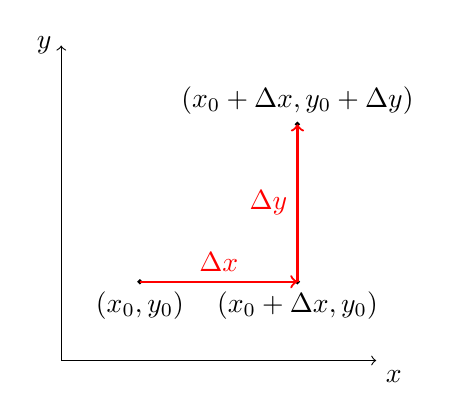
\begin{tikzpicture}
        \draw [<->] (0,4) -- (0,0) -- (4,0);
        \node [below right] at (4,0) {$x$};
        \node [left] at (0,4) {$y$};

        \draw[fill] (1,1) circle [radius=0.025];
        \draw[fill] (3,1) circle [radius=0.025];
        \draw[fill] (3,3) circle [radius=0.025];

        \node [below] at (1,1) {$(x_0, y_0)$};
        \node [below] at (3,1) {$(x_0 + \Delta x, y_0)$};
        \node [above] at (3,3) {$(x_0 + \Delta x, y_0 + \Delta y)$};

        \draw [->][thick, red] (1,1) -- node[above] {$\Delta x$} (3,1);
        \draw [->][thick, red] (3,1) -- node[left] {$\Delta y$} (3,3);
    \end{tikzpicture}
    \caption{We assume $\Delta z = f(x_0 + \Delta x, y_0 + \Delta y) - f(x_0, y_0)$ and $\Delta z = \Delta_1 z + \Delta_2 z$}
    \label{fig:proof-fundamental-lemma}
\end{figure}

\begin{enumerate}
    \item changing $x$ alone and moving from $(x_0, y_0)$ to $(x_0 + \Delta x, y_0)$, and then
    \item changing $y$ alone and moving from $(x_0 + \Delta x, y_0)$ to $(x_0 + \Delta x, y_0 + \Delta y)$
\end{enumerate}

We denote the first change in $z$ by $\Delta_1 z$, so that

\begin{equation}
    \Delta_1 z = f(x_0 + \Delta x, y_0) - f(x_0, y_0)
\end{equation}

By The Mean Value Theorem\footnote{
    \begin{Theorem}{
        The Mean Value Theorem\footnote{\href{https://trello.com/c/byu9Pyy8}{Calculus with Analytic Geometry by George F. Simmons}, p. 76}
    }{mean-value-theorem}
        Let $y = f(x)$ be a function with the following two properties:

        \begin{enumerate}
            \item $f(x)$ is continuous on the closed interval $[a, b]$; and
            \item $f(x)$ is differentiable on the open interval $(a, b)$
        \end{enumerate}

        Then there exists at least one point $c$ in the open interval $(a, b)$ such that

        \[
            f'(c) = \frac{f(b) - f(a)}{b - a}
        \]

        or equivalently,

        \[
            f(b) - f(a) = f'(c)(b - a)
        \]
    \end{Theorem}
}, we can write this as

\begin{equation}\label{eq:first-change-z-mean-val-theo}
\Delta_1 z = \Delta x f_x(x_1, y_0)
\end{equation}

where $x_1$ is between $x_0$ and $x_0 + \Delta x$. Smilary, if we denote the second part of the change in $z$ by
$\Delta_1 z$, so that

\begin{equation}
    \Delta_2 z = f(x_0 + \Delta x, y_0 + \Delta y) - f(x_0 + \Delta x, y_0)
\end{equation}

then

\begin{equation}\label{eq:second-change-z-mean-val-theo}
\Delta_2 z = \Delta y f_y(x_0 + \Delta x, y_1)
\end{equation}

where $y_1$ is between $y_0$ and $y_0 + \Delta y$.

Now as $\Delta x$ and $\Delta y \rightarrow 0$, $x_1 \rightarrow x_0$ and $y_1 \rightarrow y_0$. By the assumed
continuity of $f_x$ and $f_y$ at $(x_0, y_0)$, we can write

\begin{align}
    f_x(x_1, y_0) = f_x(x_0, y_0) + \epsilon_1 \label{eq:first-change-z-epsilon} \\
    f_y(x_0 + \Delta x, y_1) = f_y(x_0, y_0) + \epsilon_2 \label{eq:second-change-z-epsilon}
\end{align}

where $\epsilon_1$ and $\epsilon_2 \rightarrow 0$ as $\Delta x$ and $\Delta y \rightarrow 0$. Plugging
Eq.\ref{eq:first-change-z-epsilon} into Eq.\ref{eq:first-change-z-mean-val-theo} gives us

\begin{equation}
    \Delta_1 z = \Delta x\left[ f_x(x_0, y_0) + \epsilon_1 \right] = \Delta x f_x(x_0, y_0) + \Delta x\epsilon_1
\end{equation}

and similarly Eq.\ref{eq:second-change-z-epsilon} into Eq.\ref{eq:second-change-z-mean-val-theo}

\begin{equation}
    \Delta_2 z = \Delta y\left[ f_y(x_0, y_0) + \epsilon_2 \right] = \Delta y f_y(x_0, y_0) + \Delta y\epsilon_2
\end{equation}

Since we have assumed $\Delta z = \Delta_1 z + \Delta_2 z$

\begin{equation}
    \Delta z = \Delta x f_x(x_0, y_0) + \Delta x\epsilon_1 + \Delta y f_y(x_0, y_0) + \Delta y\epsilon_2 = f_x(x_0, y_0)\Delta x + f_y(x_0, y_0)\Delta y + \epsilon_1\Delta x + \epsilon_2\Delta y
\end{equation}

\qed

\footnote{\href{https://trello.com/c/byu9Pyy8}{Calculus with Analytic Geometry by George F. Simmons}, p. 681} Now Let
$f(x, y, z)$ be a function of 3 variables defined throughout some region of three-dimensional space, and let $P$ be a
point in this region. At what rate does $f$ change as we move away from $P$ in a specified direction? In the directions
of the positive x, y, and z-axes, we know that the rates of change off are given by the partial derivatives
$\frac{\partial f}{\partial x}$, $\frac{\partial f}{\partial y}$, and $\frac{\partial f}{\partial z}$. But how do we
calculate the rate of change of $f$ if we move away from $P$ in a direction that is not a coordinate direction?

Let $P = (x, y, z)$ and $\boldsymbol{R} = x\boldsymbol{i} + y\boldsymbol{j} + z\boldsymbol{k}$ being the position vector
of $P$. If we move away from $P$ to a nearby point $Q = (x + \Delta x, y + \Delta y, z + \Delta z)$, then the function
will change by an amoutn $\Delta f$. Let $\Delta s$ denote the distance between $P$ and $Q$, then we have

\begin{equation}\label{eq:def-df-over-ds}
    \frac{df}{ds} = \lim\limits_{\Delta s \rightarrow 0}\frac{\Delta f}{\Delta s}
\end{equation}

We further assume that $f(x, y, z)$ has continuous partial derivatives with respect to $x$, $y$, and $z$.

\begin{marker}
    Unless explicitly stated otherwise, all functions we deal with are always continuous in all of our discussions
\end{marker}

The \hyperlink{fundamental-lemma}{Fundamental Lemma} enables us to write $\Delta f$ in the form of

\begin{equation}\label{eq:df-in-3-partials}
    \Delta f = \frac{\partial f}{\partial x}\Delta x + \frac{\partial f}{\partial y}\Delta y + \frac{\partial f}{\partial z}\Delta z + \epsilon_1\Delta x + \epsilon_2\Delta y + \epsilon_3\Delta z
\end{equation}

As $\Delta s \rightarrow 0$, i.e. as $\Delta x \rightarrow 0$, $\Delta y \rightarrow 0$, and $\Delta z \rightarrow 0$,
$\epsilon_1, \epsilon_2, \epsilon_3 \rightarrow 0$. Dividing Eq.\ref{eq:df-in-3-partials} by $\Delta s$ gives

\begin{equation}\label{eq:df-over-ds-in-3-partials}
    \lim\limits_{\Delta s \rightarrow 0}\frac{\Delta f}{\Delta s} = \frac{\partial f}{\partial x}\frac{dx}{ds} + \frac{\partial f}{\partial y}\frac{dy}{ds} + \frac{\partial f}{\partial z}\frac{dz}{ds}
\end{equation}

Combing Eq.\ref{eq:df-over-ds-in-3-partials} and \ref{eq:def-df-over-ds} results in

\begin{equation}\label{eq:partial-chain-rule}
    \tcbhighmath[
        enhanced,colframe=red,colback=white,arc=0pt,boxrule=1pt,
        fuzzy halo=1mm with blue!50!white,
        arc=2pt,
        boxrule=0pt,
        frame hidden
    ]{
        \frac{df}{ds} = \frac{\partial f}{\partial x}\frac{dx}{ds} + \frac{\partial f}{\partial y}\frac{dy}{ds} + \frac{\partial f}{\partial z}\frac{dz}{ds}
    }
\end{equation}

\subsection{Gradient}

\footnote{\href{https://trello.com/c/U6HhhDq6}{Introduction to Electrodynamics by Griffiths, 3rd}, p. 13} The theorem
on \hyperref[eq:partial-chain-rule]{partial derivaves states} that

\begin{equation}
    dT = \left( \frac{\partial T}{\partial x} \right) dx + \left( \frac{\partial T}{\partial y} \right) dy + \left( \frac{\partial T}{\partial z} \right) dz
\end{equation}

Writing it in the dot product form:

\begin{align}
    dT &= \left( \frac{\partial T}{\partial x}\boldsymbol{\hat{x}} + \frac{\partial T}{\partial y}\boldsymbol{\hat{y}} + \frac{\partial T}{\partial z}\boldsymbol{\hat{z}} \right) \cdot (dx\boldsymbol{\hat{x}} + dy\boldsymbol{\hat{y}} + dz\boldsymbol{\hat{z}}) \\
      &= \nabla T \cdot d\boldsymbol{l} \label{eq:dt-dot}
\end{align}

where

\begin{equation}\label{eq:def-gradient}
    \nabla T \equiv \frac{\partial T}{\partial x}\boldsymbol{\hat{x}} + \frac{\partial T}{\partial y}\boldsymbol{\hat{y}} + \frac{\partial T}{\partial z}\boldsymbol{\hat{z}}
\end{equation}

is the \textbf{gradient} of $T$. We also call $\nabla$ as the \textbf{vector operator} that \textit{acts upon} $T$

\begin{tcolorbox}[
    parbox=false,
    colbacktitle=red!10!white,
    colback=blue!10!white,coltitle=red!70!black,
    title=The Geometrical Interpretation of the Gradient
]
    The doc product~\ref{eq:dt-dot} can be written as

    \begin{equation}
        dT = \nabla T \cdot d\boldsymbol{l} = \vert \nabla T \vert \vert d\boldsymbol{l} \vert \cos{\theta}
    \end{equation}

    We soon realize that the \textit{maximum} change of T occurs when $\theta = 0$, therefore

    \begin{tcolorbox}[colback=red!10!white]
        \begin{center}
            \textcolor[HTML]{8F8FF5}{\textbf{The gradient $\nabla T$ points in the direction of the maximum increase of $T$,
            and its magnitude $\vert \nabla T \vert$ gives the slope (rate of increase) along this maximal direction}}
        \end{center}
    \end{tcolorbox}
\end{tcolorbox}

Now there are 3 ways the operator $\nabla$ can act:

\begin{enumerate}
    \item On a scalar function $T$: $\nabla T$ (the gradient, which we've discussed so far)
    \item On a vector function via the dot product: $\nabla \cdot \boldsymbol{v}$ (the \textbf{divergence})
    \item On a vector function via the cross product: $\nabla \times \boldsymbol{v}$ (the \textbf{curl})
\end{enumerate}

\subsection{Divergence}

From \hyperref[eq:def-gradient]{the definition of $\nabla$}, we construct the divergence

\begin{align}
    \nabla \cdot \boldsymbol{v} &= \left( \frac{\partial T}{\partial x}\boldsymbol{\hat{x}} + \frac{\partial T}{\partial y}\boldsymbol{\hat{y}} + \frac{\partial T}{\partial z}\boldsymbol{\hat{z}} \right) \cdot (v_x\boldsymbol{\hat{x}} + v_y\boldsymbol{\hat{y}} + v_z\boldsymbol{\hat{z}}) \label{eq:divergence-dot-product} \\
    &= \frac{\partial v_x}{\partial x} + \frac{\partial v_y}{\partial y} + \frac{\partial v_z}{\partial z}
\end{align}

\subsection{Curl}

\subsubsection{The Cross Prudct of Two Vectors}

\footnote{\href{https://trello.com/c/byu9Pyy8}{Calculus with Analytic Geometry by George F. Simmons}, p. 640} Many
problems in geometry require us to find a vector that is perpendicular to each of two given vectors $\boldsymbol{A}$ and
$\boldsymbol{B}$. A routine way of doing this is provided by the \textit{cross product} (or \textit{vector product}) of
$\boldsymbol{A}$ and $\boldsymbol{B}$, denoted by $\boldsymbol{A} \times \boldsymbol{B}$. This cross product is very
different from the \hyperref[eq:divergence-dot-product]{dot product} $\boldsymbol{A} \cdot \boldsymbol{B}$, because
$\boldsymbol{A} \times \boldsymbol{B}$ is a vector while $\boldsymbol{A} \cdot \boldsymbol{B}$ is a scalar.

Consider two nonzero vectors $\boldsymbol{A}$ and $\boldsymbol{B}$. Suppose their tails conincide and let $\theta$ be
the angle from $\boldsymbol{A}$ to $\boldsymbol{B}$ (\textit{not} from $\boldsymbol{B}$ to $\boldsymbol{A}$) with
$0 \le \theta \le \pi$.

\begin{figure}[H]
    \centering
    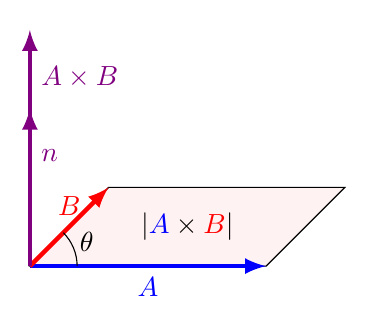
\begin{tikzpicture}
        \draw[-,fill=white!95!red](0,0)--(3,0)--(4,1)--(1,1)--cycle;
        \node at (2,0.5) {$|\textcolor{blue}{\boldsymbol{A}}\times \textcolor{red}{\boldsymbol{B}}|$};
        \draw[ultra thick,-latex,blue](0,0)--(3,0)node[midway,below]{$\boldsymbol{A}$};
        \draw[ultra thick,-latex,red](0,0)--(1,1)node[midway,above]{$\boldsymbol{B}$};
        \draw[ultra thick,-latex,blue!50!red](0,0)--(0,3)node[pos=0.8,right]{$\boldsymbol{A} \times \boldsymbol{B}$};
        \draw[ultra thick,-latex,blue!50!red](0,0)--(0,2)node[pos=0.7,right]{$\boldsymbol{n}$};
        \draw (0.6,0) arc [start angle=0,end angle=45,radius=0.6]
        node[pos=0.7,right]{$\theta$};
    \end{tikzpicture}
    \caption{The plane defined by $\boldsymbol{A}$ and $\boldsymbol{B}$}
    \label{fig:cross-prod}
\end{figure}

These 2 vectors determine a plane, as shown in Fig.~\ref{fig:cross-prod}. We now choose the unit
vector $\boldsymbol{n}$ which is normal (perpendicular) to this plane and whose direction is determined by the
\textit{right-hand thumb rule}\footnote{This means that if the right hand is placed so that the thumb is perpendicular
to the plane of $\boldsymbol{A}$ and $\boldsymbol{B}$ and the fingers curl from $\boldsymbol{A}$ to $\boldsymbol{B}$ in
the direction of angle $\theta$, then $\boldsymbol{n}$ points in the same direction as the thumb of this hand}.
\textit{This gives the direction of $\boldsymbol{A} \times \boldsymbol{B}$}

Vectors $\boldsymbol{A}$ and $\boldsymbol{B}$ also defines a parallelogram in this plane of area
$\vert \boldsymbol{A} \vert\vert \boldsymbol{B} \vert\sin{\theta}$, which defines \textit{the magnitude of
$\boldsymbol{A} \times \boldsymbol{B}$}.

\begin{Definition}{Cross Product of $\boldsymbol{A}$ and $\boldsymbol{B}$}{cross-product}
    \begin{equation}
        \boldsymbol{A} \times \boldsymbol{B} = \vert \boldsymbol{A} \vert\vert \boldsymbol{B} \vert\sin{\theta}
    \end{equation}
\end{Definition}

Our next objective is to develop a convenient formula for calculating $\boldsymbol{A} \times \boldsymbol{B}$ where

\begin{equation}\label{eq:cross-product-of-two}
    \boldsymbol{A} = a_1\boldsymbol{\hat{i}} + a_2\boldsymbol{\hat{j}} + a_3\boldsymbol{\hat{k}} \text{\ \ \ \ \ \ and \ \ \ \ \ \ }
    \boldsymbol{B} = b_1\boldsymbol{\hat{i}} + b_2\boldsymbol{\hat{j}} + b_3\boldsymbol{\hat{k}}
\end{equation}

We need to know that the cross product possesses the following algebraic properties

\begin{align}
    (c\boldsymbol{A}) \times \boldsymbol{B} &= c(\boldsymbol{A} \times \boldsymbol{B}) = \boldsymbol{A} \times (c\boldsymbol{B})\label{eq:cross-product-homogeneity}, \\
    \boldsymbol{A} \times (\boldsymbol{B} + \boldsymbol{C}) &= \boldsymbol{A} \times \boldsymbol{B} + \boldsymbol{A} \times \boldsymbol{C}\label{eq:cross-product-distributive-right}, \\
    (\boldsymbol{A} + \boldsymbol{B}) \times \boldsymbol{C} &= \boldsymbol{A} \times \boldsymbol{C} + \boldsymbol{B} \times \boldsymbol{C}\label{eq:cross-product-distributive-left}
\end{align}

Property~\ref{eq:cross-product-homogeneity}, also called \textit{homogeneous} in each
argument\footnote{\href{https://en.wikiversity.org/wiki/Cross_product}{Cross product}, Wikiversity}, is easily
established directly from Definition~\ref{def:cross-product}.

The proof of Eq.~\ref{eq:cross-product-distributive-right} starts with a unit vector $\boldsymbol{\hat{n}}$ and 3
arbitrary vectors $\boldsymbol{B}$, $\boldsymbol{C}$, and $\boldsymbol{B + C}$.
$\boldsymbol{\hat{n}} \times \boldsymbol{(B + C)}$ can be constructed by performing the following two operations:

\begin{figure}[H]
    \centering
    \begin{tikzpicture}[x=1cm, y=1cm, z=-0.6cm]
        \fill[white!95!red](-3, 0, 2.5)--(3, 0, 2.5)--(3.5, 0, -1)--(-2.5, 0, -1)--cycle;

        % Axes
        \draw [thick, -{latex[scale=3.0]}] (0,0,0) -- (0,1,0) node [at end, right] {$\boldsymbol{A}$};

        % Vectors
        \draw [very thick, -{latex[scale=3.0]}, white!45!red] (0,0,0) -- (-1,3,1)node[pos=0.7,right]{$\boldsymbol{B} + \boldsymbol{C}$};
        \draw [very thick, -{latex[scale=3.0]}, white!45!red] (0,0,0) -- (0,2,2)node[pos=0.5,below]{$\boldsymbol{B}$};
        \draw [very thick, -{latex[scale=3.0]}, white!45!red] (0,2,2) -- (-1,3,1)node[pos=0.5,left]{$\boldsymbol{C}$};

        \draw [very thick, -{latex[scale=3.0]}, white!45!red] (0,0,0) -- (-1,0,1)node[pos=1.0,above]{$(\boldsymbol{B} + \boldsymbol{C})'$};
        \draw [very thick, -{latex[scale=3.0]}, white!45!red] (0,0,0) -- (0,0,2)node[pos=0.9,below]{$\boldsymbol{B}'$};
        \draw [very thick, -{latex[scale=3.0]}, white!45!red] (0,0,2) -- (-1,0,1)node[pos=0.4,left]{$\boldsymbol{C}'$};

        \draw [very thick, -{latex[scale=3.0]}, white!45!red] (0,0,0) -- (1,0,1)node[pos=0.9,below]{$(\boldsymbol{B} + \boldsymbol{C})''$};
        \draw [very thick, -{latex[scale=3.0]}, white!45!red] (0,0,0) -- (2,0,0)node[pos=1.0,above]{$\boldsymbol{B}''$};
        \draw [very thick, -{latex[scale=3.0]}, white!45!red] (2,0,0) -- (1,0,1)node[pos=0.6,below]{$\boldsymbol{C}''$};

        % Dashes
        \draw [loosely dashed, thick] (-1,3,1) -- (-1,0,1);
        \draw [loosely dashed, thick] (0,2,2) -- (0,0,2);

        \draw [line width=0mm, white!45!red] (0, 0, 1) coordinate (a)
        -- (0, 0, 0) coordinate (b)
        -- (1, 0, 0) coordinate (c)
        pic["$\theta$", draw=black, <->, angle eccentricity=1.5, angle radius=0.3cm] {angle=a--b--c};
    \end{tikzpicture}
\end{figure}

\begin{enumerate}
    \item Project $\boldsymbol{B}$, $\boldsymbol{C}$, and $\boldsymbol{(B + C)}$ onto the plane perpendicular to
          $\boldsymbol{\hat{n}}$ to obtain a vector $\boldsymbol{B}'$, $\boldsymbol{C}'$, and $\boldsymbol{(B + C)'}$.
          By the nature of projection, the head and tails of $\boldsymbol{B'}$, $\boldsymbol{C'}$, and
          $\boldsymbol{(B + C)'}$ still coincide. Then,
    \item rotate the triangle formed by $\boldsymbol{B}'$, $\boldsymbol{C}'$, and $\boldsymbol{(B + C)'}$ by 90 degrees
          counterclockwise with respect to the tail of $\boldsymbol{\hat{n}}$ to obtain $\boldsymbol{B}''$,
          $\boldsymbol{C}''$, and $\boldsymbol{(B + C)''}$, which still form a triangle.
\end{enumerate}

Therefore, we have

\[
    (\boldsymbol{B} + \boldsymbol{C})'' = \boldsymbol{B}'' + \boldsymbol{C}''
\]

What this means is, geometrically, the operation of $\boldsymbol{\hat{n}} \times (\boldsymbol{B} + \boldsymbol{C})$ and
$\boldsymbol{\hat{n}} \times \boldsymbol{B} + \boldsymbol{\hat{n}} \times \boldsymbol{C}$ produces the same result, i.e.
the vector $(\boldsymbol{B} + \boldsymbol{C})''$. Therefore

\[
    \boldsymbol{\hat{n}} \times (\boldsymbol{B} + \boldsymbol{C}) = \boldsymbol{\hat{n}} \times \boldsymbol{B} + \boldsymbol{\hat{n}} \times \boldsymbol{C}
\]

Now let

\begin{equation}
    \boldsymbol{A} = c \boldsymbol{\hat{n}}
\end{equation}

We will then have

\[
    \cancel{\frac{1}{c}}\boldsymbol{A} \times (\boldsymbol{B} + \boldsymbol{C}) = \cancel{\frac{1}{c}}\boldsymbol{A} \times \boldsymbol{B} + \cancel{\frac{1}{c}}\boldsymbol{A} \times \boldsymbol{C}
\]

ending up with the original formula of

\[
    \boldsymbol{A} \times (\boldsymbol{B} + \boldsymbol{C}) = \boldsymbol{A} \times \boldsymbol{B} + \boldsymbol{A} \times \boldsymbol{C}
\]

\qed

Eq.~\ref{eq:cross-product-distributive-left} follows from Eq~\ref{eq:cross-product-distributive-right} combined with the
corollary of

\begin{equation}
    \boldsymbol{A} \times \boldsymbol{B} = - \boldsymbol{B} \times \boldsymbol{A}
\end{equation}

\begin{align*}
    (\boldsymbol{A} + \boldsymbol{B}) \times \boldsymbol{C} &= - \left[ \boldsymbol{C} \times (\boldsymbol{A} + \boldsymbol{B}) \right] \\
    &= - (\boldsymbol{C} \times \boldsymbol{A} + \boldsymbol{C} \times \boldsymbol{B}) \\
    &= - \boldsymbol{C} \times \boldsymbol{A} - \boldsymbol{C} \times \boldsymbol{B} \\
    &= \boldsymbol{A} \times \boldsymbol{C} + \boldsymbol{B} \times \boldsymbol{C}
\end{align*}

\qed

We continue with our task of multiplying out the \hyperref[eq:cross-product-of-two]{cross product of the vectors} using
Eq.~\ref{eq:cross-product-homogeneity},~\ref{eq:cross-product-distributive-right}, and ~\ref{eq:cross-product-distributive-left}.
By substituting $b_1\boldsymbol{\hat{i}} + b_2\boldsymbol{\hat{j}} + b_3\boldsymbol{\hat{k}}$ with $\boldsymbol{B}$:

\begin{align}
    \boldsymbol{A} \times \boldsymbol{B} &= (a_1\boldsymbol{\hat{i}} + a_2\boldsymbol{\hat{j}} + a_3\boldsymbol{\hat{k}}) \times (b_1\boldsymbol{\hat{i}} + b_2\boldsymbol{\hat{j}} + b_3\boldsymbol{\hat{k}}) \\
    &= (a_1\boldsymbol{\hat{i}} + a_2\boldsymbol{\hat{j}} + a_3\boldsymbol{\hat{k}}) \times \boldsymbol{B}\label{eq:cross-product-assumed-distributivity} \\
    &= a_1\boldsymbol{\hat{i}} \times \boldsymbol{B} + a_2\boldsymbol{\hat{j}} \times \boldsymbol{B} + a_3\boldsymbol{\hat{k}} \times \boldsymbol{B} \\
    &= a_1\boldsymbol{\hat{i}} \times (b_1\boldsymbol{\hat{i}} + b_2\boldsymbol{\hat{j}} + b_3\boldsymbol{\hat{k}}) + a_2\boldsymbol{\hat{j}} \times (b_1\boldsymbol{\hat{i}} + b_2\boldsymbol{\hat{j}} + b_3\boldsymbol{\hat{k}}) + a_3\boldsymbol{\hat{k}} \times (b_1\boldsymbol{\hat{i}} + b_2\boldsymbol{\hat{j}} + b_3\boldsymbol{\hat{k}}) \\
    &= a_1 b_1 \boldsymbol{\hat{i}} \times \boldsymbol{\hat{i}} + a_1 b_2 \boldsymbol{\hat{i}} \times \boldsymbol{\hat{j}} + a_1 b_3 \boldsymbol{\hat{i}} \times \boldsymbol{\hat{k}} + a_2 b_1 \boldsymbol{\hat{j}} \times \boldsymbol{\hat{i}} + a_2 b_2 \boldsymbol{\hat{j}} \times \boldsymbol{\hat{j}} + a_2 b_3 \boldsymbol{\hat{j}} \times \boldsymbol{\hat{k}} + a_3 b_1 \boldsymbol{\hat{k}} \times \boldsymbol{\hat{i}} + a_3 b_2 \boldsymbol{\hat{k}} \times \boldsymbol{\hat{j}} + a_3 b_3 \boldsymbol{\hat{k}} \times \boldsymbol{\hat{k}}\label{eq:cross-product-complete-expand}
\end{align}

With the following corollaries,

\begin{align}
    \boldsymbol{\hat{i}} \times \boldsymbol{\hat{i}} = 0 \\
    \boldsymbol{\hat{j}} \times \boldsymbol{\hat{j}} = 0 \\
    \boldsymbol{\hat{k}} \times \boldsymbol{\hat{k}} = 0 \\
    \boldsymbol{\hat{i}} \times \boldsymbol{\hat{j}} = -\boldsymbol{\hat{j}} \times \boldsymbol{\hat{i}} = \boldsymbol{\hat{k}} \\
    \boldsymbol{\hat{j}} \times \boldsymbol{\hat{k}} = -\boldsymbol{\hat{k}} \times \boldsymbol{\hat{j}} = \boldsymbol{\hat{i}} \\
    \boldsymbol{\hat{k}} \times \boldsymbol{\hat{i}} = -\boldsymbol{\hat{i}} \times \boldsymbol{\hat{k}} = \boldsymbol{\hat{j}} \\
\end{align}

Eq.~\ref{eq:cross-product-complete-expand} simplifies down to

\begin{align}
    \boldsymbol{A} \times \boldsymbol{B} &= a_1 b_2 \boldsymbol{\hat{k}} - a_1 b_3 \boldsymbol{\hat{j}} - a_2 b_1 \boldsymbol{\hat{k}} + a_2 b_3 \boldsymbol{\hat{i}} + a_3 b_1 \boldsymbol{\hat{j}} - a_3 b_2 \boldsymbol{\hat{i}} \\
    &= (a_2 b_3 - a_3 b_2)\boldsymbol{\hat{i}} - (a_1 b_3 - a_3 b_1)\boldsymbol{\hat{j}} + (a_1 b_2 - a_2 b_1)\boldsymbol{\hat{k}}\label{eq:cross-product-algebraic-expand}
\end{align}

We recall that a determinant of order 2 is defined by

\begin{equation}
    \begin{vmatrix}
        a_1 & a_2 \\
        b_1 & b_2 \\
    \end{vmatrix} = a_1 b_2 - a_2 b_1
\end{equation}

A determinant of order 3 can be defined in terms of determinants of order 2 as

\begin{equation}
    \begin{vmatrix}
        a_1 & a_2 & a_3 \\
        b_1 & b_2 & b_3 \\
        c_1 & c_2 & c_3 \\
    \end{vmatrix} =
    a_1 \begin{vmatrix}
        b_2 & b_3 \\
        c_2 & c_3 \\
    \end{vmatrix} -
    a_2 \begin{vmatrix}
        b_1 & b_3 \\
        c_1 & c_3 \\
    \end{vmatrix} +
    a_3 \begin{vmatrix}
        b_1 & b_2 \\
        c_1 & c_2 \\
    \end{vmatrix}
\end{equation}

Eq.~\ref{eq:cross-product-algebraic-expand} is equivalent to

\begin{align}
    \boldsymbol{A} \times \boldsymbol{B} &=
    \begin{vmatrix}
        a_2 & a_3 \\
        b_2 & b_3 \\
    \end{vmatrix} \boldsymbol{\hat{i}} -
    \begin{vmatrix}
        a_1 & a_3 \\
        b_1 & b_3 \\
    \end{vmatrix} \boldsymbol{\hat{j}} +
    \begin{vmatrix}
        a_1 & a_2 \\
        b_1 & b_2 \\
    \end{vmatrix} \boldsymbol{\hat{k}} \\ &=
    \begin{vmatrix}
        \boldsymbol{\hat{i}} & \boldsymbol{\hat{j}} & \boldsymbol{\hat{j}} \\
        a_1 & a_2 & a_3 \\
        b_1 & b_2 & b_3 \\
    \end{vmatrix} \label{eq:cross-product-algebraic-form}
\end{align}

\begin{tcolorbox}[
    parbox=false,
    enhanced,
    colback=red!5!white,colframe=red!75!black,
    watermark tikz={\draw[line width=2mm] circle (1cm) node{\fontfamily{ptm}\fontseries{b}\fontsize{20mm}{20mm}\selectfont !};}
]
    It should be noted that formula~\ref{eq:cross-product-algebraic-form} is by no means a definition of cross product,
    because obtaining it must assume the \hyperref[eq:cross-product-assumed-distributivity]{distributivity law}
    \footnote{\href{https://math.stackexchange.com/questions/362139/how-to-prove-the-distributive-property-of-cross-product\#comment5670827\_362161}{The determinant pre-assumes the distributivity of cross product}}.
    We should view \ref{eq:cross-product-algebraic-form} simply as a convenient tool for making calculations

    In addition, Definition like \ref{def:cross-product} that avoid dependence on explicit representations of vectors in
    terms of any particular coordinate system are called \textit{invariant} or \textit{coordinate-free}.
    \ref{eq:cross-product-algebraic-form} doesn't preserve such invariant because it assumes a Cartesian
    space\footnote{\href{https://en.wikiversity.org/wiki/Cross_product\#Algebraic\_Definition}{Cross product}, Wikiversity}
\end{tcolorbox}